\documentclass[11pt, oneside]{article} 	% use "amsart" instead of "article" for AMSLaTeX format
\usepackage{geometry} 		% See geometry.pdf to learn the layout options. There are lots.
\geometry{letterpaper}  		% ... or a4paper or a5paper or ... 
\usepackage[parfill]{parskip} 		% Activate to begin paragraphs with an empty line rather than an indent
\usepackage{graphicx}				% Use pdf, png, jpg, or eps§ with pdflatex; use eps in DVI mode
								% TeX will automatically convert eps --> pdf in pdflatex		
\usepackage{amssymb}
\usepackage{amsmath}
\usepackage{authblk}
\usepackage[
backend=biber,
style=alphabetic,
]{biblatex}
\usepackage{graphicx}
\graphicspath{ {./images/} }
\usepackage{verbatim}
\usepackage{tikz} 
\usepackage{subfig}

\usepackage{syntonly}
% \syntaxonly <-- use this for checking syntax only
% \mbox {text} - keep together
% \fbox {text} - keep together and draw around

%\pagestyle{plain|headings|empty} % header and footer p.27
%SetFonts
%\include{filename}, \includeonly{filename1, filename2} , \input[fiename}

%SetFonts% 

\title{The Office DVD Problem}
\author{Dave Fetterman}
\affil{Obviously Unemployed}
\date{7/10/22}
\begin{document}
\maketitle

Screensavers have captivated [this] man since the 1990s. If watched long enough, what will the spirits of the machine tell us?

Specifically, the question of whether a bouncing rectangle will slide \emph{exactly} into the corner of the screen, for a satisfying, perfectly diametric rebound, was even addressed on \emph{The Office}:
\url{https://www.youtube.com/watch?v=QOtuX0jL85Y}

However, though these characters reportedly watched this sleep-mode drama play out for years until payoff, we ask - under what conditions \emph{will} the rectangle perfectly bounce into the screen's corner?
 
\begin{figure}
\centering
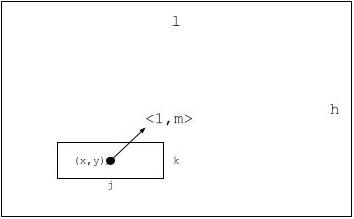
\includegraphics[scale=.5]{setup}
\caption{The Office DVD problem's most generic setup}
\end{figure}

\subsection{Statement} 
Suppose we have a screen of length $l$, height $h$, containing an axis-aligned rectangle of length $j$ and height $k$ centered at point $(x, y)$.

Suppose this rectangle is launched at direction $\langle 1, m\rangle$ \footnote {Think of this as slope $m$} and ``bounces'' according to billiard rules \footnote{Glancing off a horizontal boundary, our trajectory goes from $\langle 1, m \rangle$ to $\langle 1, -m \rangle$, with $\langle \pm 1, m \rangle$ to $\langle \mp 1, m \rangle$ for horizontal}.

Given $l, h, j, k, m \in \mathbb{R}$, can we tell whether the rectangle ever bounce perfectly into a corner?  

We can approach this problem from the simplest version to the most complex.

\subsection{Problem 1} 

Suppose $j = k = 0$ and $x = y = 0$. In other words, suppose we have a \emph{point} starting at the corner
 (origin).  Under what conditions does this bounce into a corner?


\subsection{Problem 2} 

Suppose $j, k > 0, x = \frac{j}{2}, y = \frac{k}{2}$. In other words, suppose we have a rectangle starting at the corner. Under what conditions does this bounce into a corner?

\subsection{Problem 3} 

Suppose we have maximally open (reasonble) conditions, with $x \in [\frac{j}{2}, l - \frac{j}{2}], y \in [\frac{k}{2}, h - \frac{k}{2}]$. Under what conditions does this bounce into a corner?


\section{Solutions}

Note: If our initial slope is zero $m = \langle 1, 0 \rangle$ or ``infinite'' (sort of disallowed in setup), the solution is trivial: if we're in a corner now, we'll be in one shortly, otherwise we never will.s

Note also that, for the sake of simplicitly, we can treat $m$ as always positive (going up and to the right).  If not, inverting the problem ($m \rightarrow -m, y = h - y)$ yields the same answer.  The box initially moving leftwards (disallowed in the problem) submits to the same kind of reduction by the same sort of symmetry.

\subsection{Problem 1 solution}

The key insight here is that though the point bounces "within a box" until meeting $(0,0), (0, h), (l, 0), $ or $(l, h)$, (as in Figure 2) we can instead look at the path of the point in an unconstrained space, seeing if we hit a point of the form $a \cdot l, b \cdot h$ with $a,b \in \mathbb{N}$.

\begin{figure}[!htb]
\centering
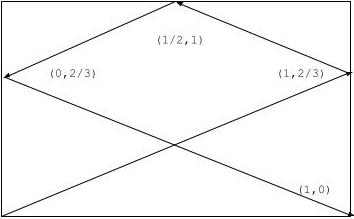
\includegraphics[scale=.5]{problem1trajectory}
 \caption{Sol 1:Success for $m = \frac{2}{3}, h, l = 1, j, k = 0$}
\end{figure}

Consider that, on meeting the point $(0, \frac{2}{3})$, we can either consider what happens if we reflect "back" as in Figure 2, or, equivalently, if we pass "through" as in Figure 3.  We quickly see that:



\begin{itemize} 
\item If the left-hand side meets a corner, the mirror-image on the right-hand side will meet a corner.
\item Likewise for the converse: the right meeting a corner means the left has as well.
\item If the left-hand side does \emph{not} meet a corner, the right-hand side cannot.
\item Likewise for the converse.
\end{itemize}


\begin{figure}[!htb]
\centering
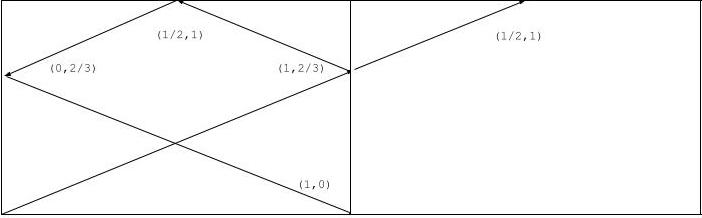
\includegraphics[scale=.5]{mirrorright}
 \caption{Sol 1: TODO}
\end{figure}

This applies for top-bottom just as easily as left-right.

\begin{figure}[!htb]
\centering
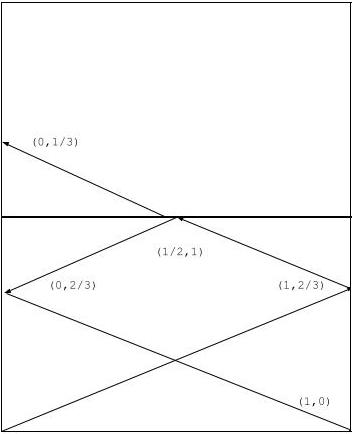
\includegraphics[scale=.5]{mirrorup}
 \caption{Sol 1: TODO}
\end{figure}

Therefore, composing these two, we can cast the path of the smaller rectangle as entirely ``up and to the right''.  

\begin{figure}[!htb]
\centering
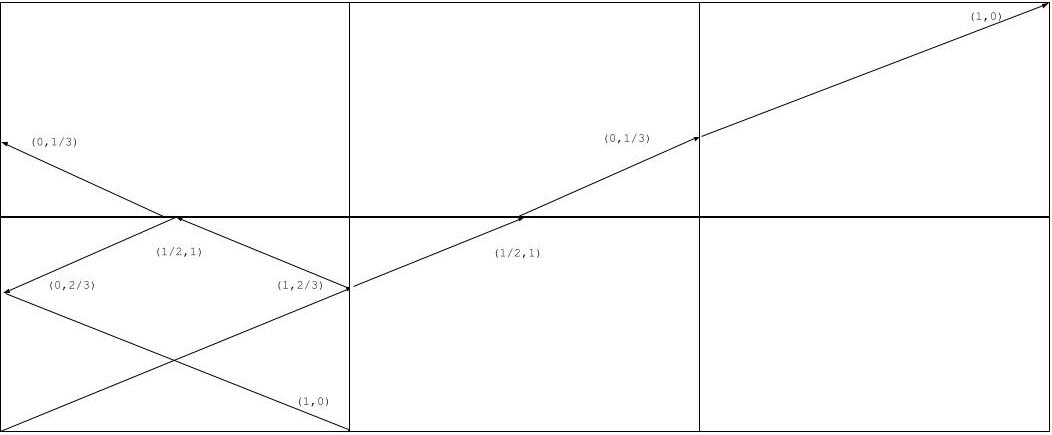
\includegraphics[scale=.4]{fullpath}
 \caption{Sol 1: TODO}
\end{figure}




TODO TODO TODO TODOT

\subsection{Problem 2 solution}

The key insight here is that instead of each ``frame'' extending from $(0, 0)$ to $(l, h)$, with the box's center ($x, y)$ constrained to the rectangle defined by $[\frac{j}{2}, l - \frac{j}{2}], \times [\frac{k}{2}, h - \frac{k}{2}]$, we can instead treat the \emph{center} of that $[\frac{j}{2}, l - \frac{j}{2}], \times [\frac{k}{2}, h - \frac{k}{2}]$ box as a point like in problem 1.  

It is then clear that we can use problem 1's main insight to the center point as opposed to the small rectangle: that the small rectangle, say, $\frac{j}{2}$ left of the right border of one frame will take an equivalent trajectory to one $\frac{j}{2}$ right of the left border of the adjoining right frame.

So, restate the problem as $j, k = 0, x \rightarrow x - \frac{j}{2} y \rightarrow \frac{k}{2}$ and solve as in problem 1.

\begin{figure}[!htb]
\centering
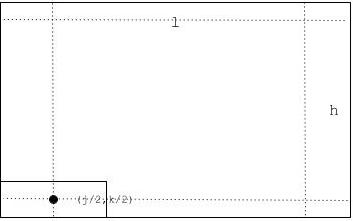
\includegraphics[scale=.5]{problem2}
\end{figure}




\end{document}
